% Compile with: latexmk -pdfxe -outdir=build
\documentclass[12pt,oneside]{LuThesis}
\usepackage{graphicx}

\title{Saules paneļu efektivitāte Latvijas klimatā}
\author{Viktorija Leimane}

%%% LuThesis deklerācijas
\def\studaplnum{vl16047}
\def\darbvad{Dr. Phys. Andris Jakovičs}
\def\dokfak{\textbf{Fizikas, matemātikas un optometrijas fakultāte}}
\def\recenzents{Dr. Phys.Aivars Vembris}
\def\doktitle{\textbf{Saules paneļu efektivitāte Latvijas klimatā}}
\def\dokfak{\textbf{Fizikas, matemātikas un optometrijas fakultāte}}
\def\dokdate{} % Darba vadītāja parakstīšanas datums
\def\dokdateiesn{} % Darba iesniegšanas datums

%%% Valodas un fonti
\setdefaultlanguage{latvian}
\setotherlanguage{english}
\setmainfont[BoldFont=FreeSerifBold.ttf,ItalicFont=FreeSerifItalic.ttf,BoldItalicFont=FreeSerifBoldItalic.ttf]{FreeSerif.ttf}

%%% Misc
\usepackage{hyperref}
\addbibresource{bachelor.bib} % biblatex bibliotēkas fails: bachelor.bib

%%% Dokumenta struktūra
\begin{document}

\maketitle

% * Anotācija
\chapter*{Anotācija}
\setcounter{page}{1}
\begin{abstract}
Darba mērķis ir noteikt efektīvāko saules paneļu izvietojuma veidu Latvijas klimatiskajos apstākļos. 
Balstoties uz divu veidu saules paneļiem, kas novietoti piecās dažādās telpiskajās orientācijās Latvijas Universitātes Botāniskā dārza teritorijā, tiek noteikta solāro paneļu efektivitātes atkarība no mainīgiem parametriem:
\begin{enumerate}
\item solāro paneļu tips
\item telpiskā orientācija
\item gada mēnesis
\item meteoroloģiskie apstākļi.
\end{enumerate}

Iegūtie monitoringa rezultāti tiek analizēti kontekstā ar saules izstarojuma intensitāti, paneļu parciālās(?) efektivitātes fizikālo novērtējumu un citu mērījumu rezultātiem.\\

\keywords{Saules enerģijas paneļi, atjaunojamo energoresursu enerģija}
\end{abstract}

\chapter*{Abstract}
\begin{english}
\begin{abstract}
The aim of this thesis is to determine optimal solar panel arrangement for the climatic conditions of Latvia.
By studying two types of solar panels placed in five different spatial orientations in the University of Latvia Botanical Garden area, the dependency of solar panel efficiency on following variable parameters is established:
\begin{enumerate}
\item Type of solar panels (JA or LG)
\item Spatial orientation (W.13, E.13, S.13, S.40, S.90)
\item Month of year (january - april)
\item Meteorological conditions (solar irradiance and clouds)
\end{enumerate}

The results of the monitoring are analysed in the context of solar irradiance intensity, the physical assessment of the potential efficiency of the panels and the results of other measurements.
The results show that the optimal parameters are LG panel at a direction south 40 degree angle. The study data analysis tool is available in \url{https://github.com/chararchter/solR}.

\keywords{Solar panels, renewable energy}
\end{abstract}
\end{english}

%* Saturs
\tableofcontents

%* Apzīmējumu saraksts
\chapter*{Apzīmējumu saraksts}
\addcontentsline{toc}{chapter}{Apzīmējumu saraksts}
\noindent 
\textbf{Klimats}\\
TSI - Kopējais saules apstarojums, $\textrm{Wm}^{-2}$\\
SSI - Saules spektrālais apstarojums, $\textrm{Wm}^{-2}\textrm{nm}^{-1}$\\
% $G_{sc}$ - Solārā konstante, $\textrm{Wm}^{-2}$\\
%Photovoltaic power potential
TIM - Kopējā apstarojuma novērotājs\\
GHI – Globālais horizontālais apstarojums,  $\textrm{kWh/m}^2$\\ %Global horizontal irradiation
DHI – Difūzais horizontālais apstarojums,  $\textrm{kWh/m}^2$\\ 
DNI – Tiešais normālais apstarojums, $\textrm{kWh/m}^2$\\ %Direct normal irradiation
CMF - Mākoņu modifikācijas reizinātājs\\
AU - astronomiskā vienība\\  %astronomical unit
\textbf{Saules kustības leņķi}\\
$\theta$ - staru krišanas leņķis uz saules paneli\\
$\delta$ - Saules deklinācija -- leņķis starp virzieniem uz Sauli un debess ekvatoru solārajā pusdienlaikā.\\
 $\phi$  - ģeogrāfiskais platums; pozitīvs Z virzienā.\\
$\beta$  - paneļa slīpums -- leņķis starp Saules paneļa virsmu un horizontāli.\\
$\gamma$ - paneļa azimuts -- leņķis starp virsmas normāles projekciju uz horizontālo  plakni un D virzienu.\\
$\omega$ - solārais stundu leņķis -- leņķis starp Saules stara virziena projekciju uz horizontālo plakni un D virzienu; negatīvs no rīta.\\
\textbf{Saules paneļi}\\
PV - fotoelektriskais elements\\ %fotogalvanisks?
Si - silīcijs\\
P - jauda, 	W\\
Pmax - maksimālā jauda, W\\
PVOUT – Saules fotoelementa potenciālā jauda, $\textrm{kWh/kWp}$\\ 
%Photovoltaic power potential
E$_{norm}$, $\textrm{kWh/m}^2$ - enerģija normēta uz saules paneļa laukuma vienību.\\
\textbf{Debespuses}\\
A - austrumi\\
R - rietumi\\
D - dienvidi\\

%* Ievads
\chapter*{Ievads}
\addcontentsline{toc}{chapter}{Ievads}
Apvienoto Nāciju Organizācijas Klimata konferencē Parīzē 2015. gada decembrī daudzas pasaules valstis vienojās ierobežot globālo sasilšanu zem 2 ºC salīdzinājumā ar pirmsindustriālo laikmetu.
%, tāpēc ES ir apņēmusies līdz 2030. gadam samazināt siltumnīcefekta gāzu emisijas vismaz par 40\% salīdzinājumā ar 1990. gada līmeni.
Tāpēc Eiropas Savienībā noteikts dalībvalstīm saistošs mērķrādītājs  –  vismaz 32\%  atjaunojamās enerģijas īpatsvars līdz 2030. gadam \cite{ES}.

Ne mazāk būtiska ir atjaunojamo energoresursu loma energoapgādes neatkarības un drošības veicināšanā, tehnoloģiju attīstībā un inovācijās, vienlaikus sniedzot labumu videi un sabiedrībai, kā arī nodrošinot svarīgus priekšnosacījums nodarbinātībai, reģionālajai attīstībai un elektrības nodrošināšanai grūti pieejamās vietās \cite{ES}.

Dažādu pieejamo atjaunojamo resursu - Saule, vējš, zeme, ūdens - starpā Saules enerģija ir viens no kandidātiem klimata pārmaiņu un to seku mazināšanai un efektīvas energoapgādes nodrošināšanai. Pēdējā desmitgadē veiktās investīcijas Saules enerģijas izmantošanā manifestējās inovācijās saules paneļu ražošanā, un gala rezultātā tie ir kļuvuši efektīvāki un finansiāli pieejamāki patērētājiem, piemēram, rakstā \cite{researchOpp} norādīts, ka silīcija saules paneļu cena sastāda mazāk nekā 30\% no kopējām saules paneļu sistēmas uzstādīšanas izmaksām un to saražotā enerģija atmaksājas vidēji trīs gadu periodā.

Tomēr bez klimata to efektivitāti ietekmē arī daudzi citi faktori, to skaitā telpiskā orientācija.

Šī pētījuma \textbf{mērķis} ir analizēt un praktiski pārbaudīt divu tipu (JA un LG) saules paneļu efektivitāti atšķirīgos telpiskās orientācijās risinājumos -- pētītas trīs dažādu virzienu (dienvidi, rietumi, austrumi) un trīs leņķu (13, 40, 90) paneļu grupas -- un tiek salīdzināta to piemērotība Latvijas klimatiskajiem apstākļiem.

\textbf{Darba uzdevumi}
\begin{itemize}
\item Ievākt, atlasīt un analizēt saules paneļu datus.
\item Izveidot iespējami automatizētu datu apstrādes sistēmu R valodā ilgtermiņa montioringa vajadzībām.
\item Salīdzināt paneļu efektivitāti mēnešu un gada laikā atbilstoši to parametru (paneļu tipa un telpiskās orientācijas) apakšklasēm.
% \item Balstoties uz ilgtermiņa saules izstarojuma monitoringu, novērtēt saules paneļu saražoto enerģiju no fizikālajiem apsvērumiem.
\item Novērtēt datu kvalitāti no fizikālo apsvērumu un citu mērījumu viedokļa.
\end{itemize}

\textbf{Darba struktūra}\\
Darba pirmo daļu veido literatūrā pieejamo Saules apstarojuma novērtējumu raksturojums un apskata par Saules redzamo pārvietošanās pie debess sfēras diennakts laikā janvāra un aprīļa mēnešos. Otrajā daļā aplūkota saules paneļu uzbūve un darbības princips, kā arī apskatīta sistēmas shēma un saues paneļu konkrētās instalācijas LU Botāniskajā dārzā parametru raksturojums.
Trešā daļā ir aprakstīti iegūtie rezultāti, tie ir salīdzināti savā starpā, ar cita saules paneļa uzstādījuma mērījumu rezultātiem un 


ar eksperimentālā poligona meteostacijas datiem par solāro apstarojumu šajā laika periodā.


% un lai to analīzi veiktu ir darīti uzdevumi
% uzstādīti paneļi (profesionāļi to darīja)
% Ievākti un analizēti dati
% Datu kvalitātes novērtējums
% novērtēt vai iegūtie resultāti ir ticami

% citos klimatiskajos apstākļos līdzīgas analīzes ir veiktas ko var iegūt dažādās klimatiskajās zonās 
% pierakstīt par pv paneļu darbību un efektivitāti
% aprakstīt ko tu darīji, lai pēc iespējas automatizētu datu apstrādes sistēmu
% kādus datus uzkrāj kādā attēlojumā
% datu menedžmentu aprakstīt
% TEORIJAS KOPSAVILKUMS
Vispirms tiek aplūkota Saules emitētā starojuma daba un ģeometriskie apsvērumi - virziens, no kura staru kūlis sasniedz virsmu, leņķis uz virsmas un laika gaitā saņemtais starojuma daudzums. Tiek apskatīta atmosfēras ietekme uz virsmas saņemto saules starojumu, un tās praktiskā nozīme, apstrādājot pieejamos Saules starojuma datus, lai aprakstītu radiācijas gadījumus uz virsmas dažādās orientācijās.

% * Literatūras apskats
\chapter{Literatūras apskats}
\input{tex/literatura}
\section{Saules apstarojums}

Lielākā daļa Saules emitētās enerģijas tiek saražota kodolreakcijās fotosfērā. 
Kopējais saules apstarojums (TSI) raksturo Saules starojuma absolūto intensitāti,
enerģiju uz virsmas perpendikulāri starojuma izplatīšanas virzienam 1 AU attālumā no Saules, integrēta visā saules enerģijas diskā un visā saules enerģijas spektrā. \cite{ThermalProcesses} TSI vērtībai novērojama aptuveni 11 gadus ilga periodiska variācija, kas korelē ar saules plankumu skaitli (\ref{fig:TSI_misijas}. att.)  un norāda uz solārās radiācijas izmaiņām, kas ietekmē saņemto solārās enerģijas apjomu uz Zemes atmosfēras augšējiem slāņiem. Papildus ir noderīgi zināt saņemtā starojuma spektrālo sadalījumu (SSI) -- ~\ref{fig:SSI}. attēlā redzams, ka aptuveni puse starojuma tiek saņemta 380 -- 780 nm diapazonā, kas padara iespējumu no tā iegūt enerģiju ar saules paneļu paņēmienu.

TSI novērojumi no kosmosa tiek veikti kopš 1978. gada un instrumentu specifikas dēļ iegūtas dažādas absolūtās vērtības (\ref{fig:TSI_misijas}. att.), tāpēc šī fizikālā lieluma tikai daļēji pārkājušos novērojumu laikrindu apvienošana kompozītā ir gan zinātnisks, gan statistisks izaicinājums un neviens kompozīts (piemēram, PMOD, ACRIM, IRBM) līdz šim nav guvis konsensu solārā apstarojuma pētnieku kopienā.

\begin{figure}[h]
    \centering
    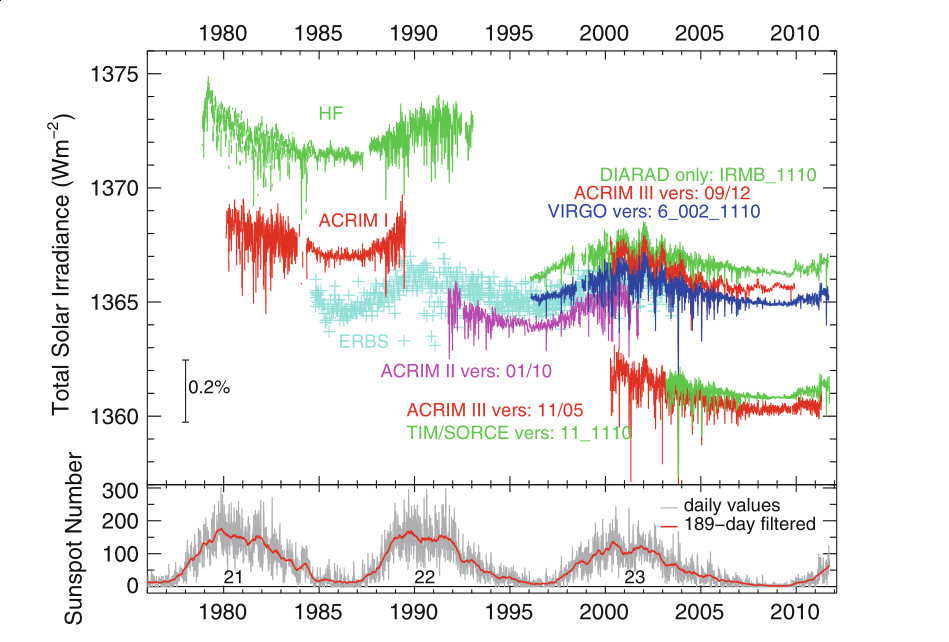
\includegraphics[width=0.6\linewidth]{figures/misc/TSI_misijas.png}
    \caption{Salīdzinājums dienā vidējotiem saules kopējā apstarojuma datiem no dažādām misijām un Saules plankuma skaitlis, lai ilustrētu solārās aktivitātes variabilitāti trīs ciklos. \cite{Frohlich2012}}
    \label{fig:TSI_misijas}
\end{figure}

% \begin{table}[h]
%     \caption{TSI mērījumu vēsture} % uzrakstīt kādu absolūto TSI izmērīja vai norādīt uz grafiku?
%     \begin{center}
%     \begin{tabular}{| r | c | l |}
%     \hline
%     radiometrs & misija & darbības laiks \\ \hline
%     Hickey-Frieden & NIMBUS-7 & 1978--1992  \\ \hline
% 	ACRIM I & Solārā Maksimuma Misija (SMM) & 1980--1989 \\ \hline
% 	ACRIM  & Zemes Radiācijas Budžeta Satelīts (ERBS) & 1984--2003 \\ \hline
% 	ACRIM II & Augšējās Atmosfēras Izpētes Satelīts (UARS) & 1991--2001 \\ \hline
% 	VIRGO & Solārā un Heliosfēras observatorija (SOHO)& 1996--pašlaik \\ \hline
% 	ACRIM III & ACRIMSAT  & 2000--pašlaik \\ \hline
% 	TIM & Saules Radiācijas un Klimata Eksperiments (SORCE) & 2003--pašlaik\\ \hline
%     \end{tabular}
%     \end{center}
%     \label{tab:radiometers}
% \end{table}

Par labāko saules apstarojuma mērījumu reprezentāciju tiek uzskatīti TIM instrumenta dati mēraparāta uzbūves (atšķirībā no citiem radiometriem TIM precizitātes apertūra atrodas tuvu dobumam un redzeslauku bloķējošā apertūra ir pie instrumenta ieejas) un augstās precizitātes -- nenoteiktība tiek novērtēta esam mazāk nekā $0.014\textrm{Wm}^{-2}\textrm{yr}^{-1}$ un precizitāte ar $0.48\textrm{Wm}^{-2}$ \cite{TSIdata} -- dēļ, tāpēc šajā darbā grafiki balstās uz šiem mērījumiem, pēc kuriem absolūtā kopējā saules apstarojuma vērtība ir $1360.8 \pm 0.5 \textrm{Wm}^{-2}$.\cite{Frohlich2012}

\begin{figure}[h]
    \centering
    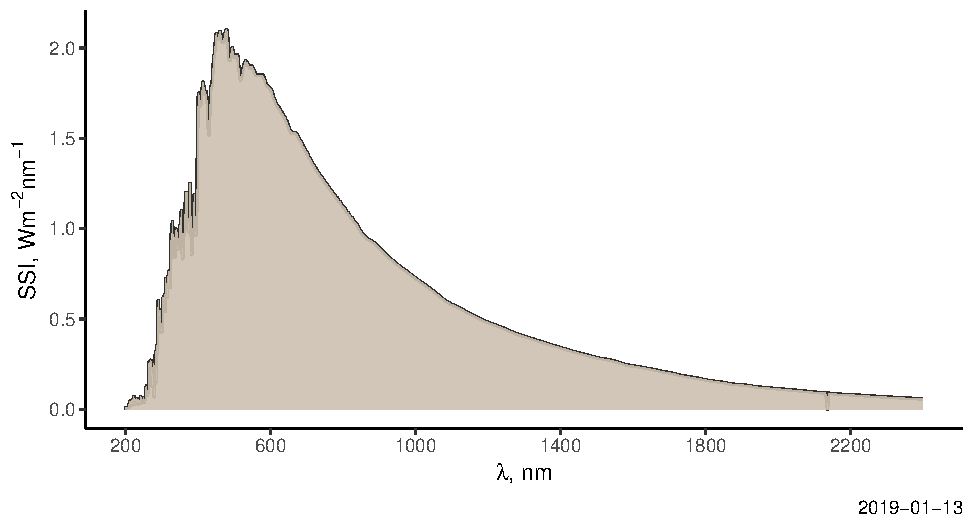
\includegraphics[width=\linewidth]{figures/misc/SSI.pdf}
    \caption{SSI 1AU attālumā (24 h vidējā vērtība) \cite{SSIdata}}
    \label{fig:SSI}
\end{figure}

\begin{figure}[h]
    \centering
    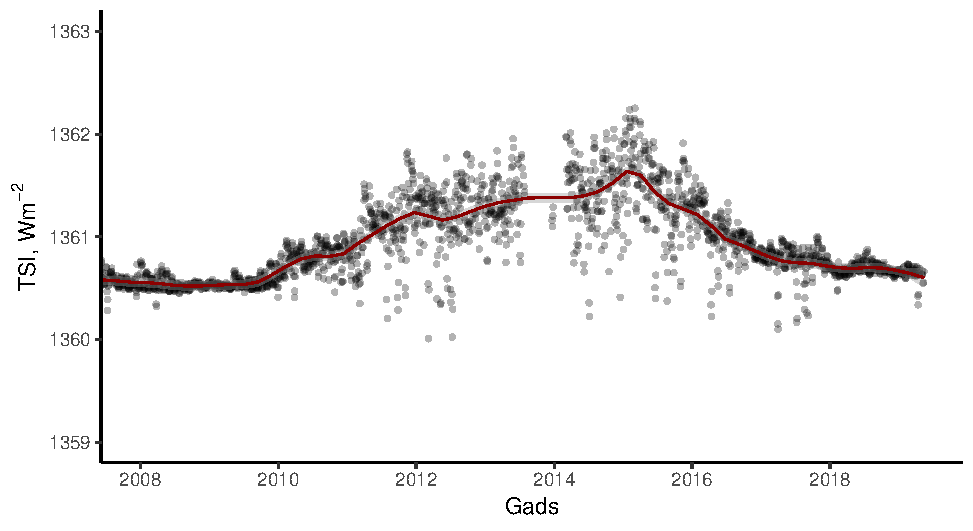
\includegraphics[width=\linewidth]{figures/misc/TSI_8-19.pdf}
    \caption{TSI 24. saules ciklā 1AU attālumā (24 h vidējā vērtība)\cite{TSIdata}}
    \label{fig:TSI1}
\end{figure}

\begin{figure}[h]
    \centering
    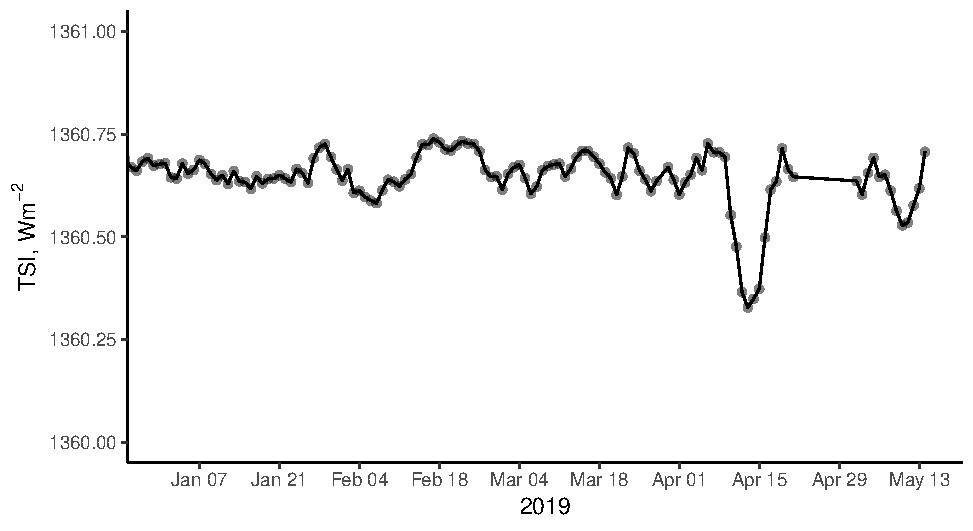
\includegraphics[width=\linewidth]{figures/misc/TSI.pdf}
    \caption{TSI izmaiņas solāro paneļu datu ieguves laikā 1AU attālumā (24 h vidējā vērtība)\cite{TSIdata}}
    \label{fig:TSI2}
\end{figure}

% \begin{figure}[h]
%     \centering
%     \includegraphics[width=\linewidth]{figures/misc/LV_DNI.png}
%     \caption{Tiešais normālais apstarojums \cite{solargis}}
%     \label{fig:lv_DNI}
% \end{figure}
% \begin{figure}[h]
%     \centering
%     \includegraphics[width=\linewidth]{figures/misc/LV_GHI.png}
%     \caption{Globālais horizontālais apstarojums Latvijā \cite{solargis}}
%     \label{fig:lv_GHI}
% \end{figure}
% \begin{figure}[h]
%     \centering
%     \includegraphics[width=\linewidth]{figures/misc/LV_PVOUT.png}
%     \caption{PV potenciālā jauda \cite{solargis}}
%     \label{fig:lv_PVOUT}
% \end{figure}


%* Rezultāti
\chapter{Rezultāti un diskusija}
\input{tex/rezultati}

%* Secinājumi
\chapter*{Secinājumi}
\addcontentsline{toc}{chapter}{Secinājumi}
Darba laikā tika izveidota programmatūra, ar kuras palīdzību tika atlasīts, analizēts un apkopots liels datu apjoms par 10 saules paneļu darbību no 2019. gada 1. janvāra līdz 30. aprīlim. Pētījuma datu analīzes rīks ir pieejams \url{https://github.com/chararchter/solR}.

Darbā iegūtie rezultāti ļauj izdarīt secinājumus, ka no sistēmā esošajiem parametriem efektīvākā kombinācija ir:
\begin{itemize}
	\item 40 grādu leņķis
	\item D virziens
	\item LG panelis
	\item aprīļa mēnesis
\end{itemize}

% KĻŪDAS!!!?????????

Saules paneļu efektivitātes citu faktoru ietekmes izpratne prasa turpmākus pētījumus, it īpaši nolietojuma, putekļu, vēja, nokrišņu un citu apstākļu ietekmes izvērtēšanai. Lai iegūtu datus un veiktu analīzi pilna gada periodam, šo montiroingu ir paredzēts turpināt vismaz trīs gadus.

%* Pateicības
\chapter*{Pateicības}
\addcontentsline{toc}{chapter}{Pateicības}
Pateicos paroksetīnam, xanax, GNU/Linux, Pētera Draguna dzejas krājumam 'Tumšās stundas', Tarvi Verro for teaching me git, Valtam Krūmiņam un Annai Bulei par emocionālo atbalstu, Paulīnai Lodbrukai un Pēterim Ratniekam par ticību maniem spēkiem, Žeņam par kucēnu video, Solvitai par maģiju un Cilvēkam par pacietību. Paldies Aleksandrai Elbakjanai par sci-hub. Paldies "Puratos Latvia" un Asjas un Berndta Everts piemiņas fondam par stipendiju studiju laikā.\\

Darbs veikts ar Eiropas Reģionālās attīstības fonta projekta "Viedo risinājumu gandrīz nulles enerģijas ēkām izstrāde, optimizācija un ilgtspējas izpēte reāla klimata apstākļos" Nr ESS2017/209 1.1.1.1/16/A/192 finansiālo atbalstu.


%* Izmantotā darba literatūra un avoti
\clearpage
\addcontentsline{toc}{chapter}{Izmantotā darba literatūra un avoti}
\printbibliography[title=Izmantotā darba literatūra un avoti]

%%% Pielikumi
\appendix

% Dokumentālā lapa
\makedoklapa

\end{document}
